\documentclass[10pt,oneside,a4paper, english]{article}
\usepackage[T1]{fontenc}
\usepackage[latin2, utf8]{inputenc}
\usepackage[english]{babel}
\usepackage{listings}
\usepackage{color}
\usepackage[margin=3cm]{geometry}
\usepackage{titlesec}
\usepackage{changepage}
\usepackage{enumitem}
\usepackage{graphicx}
\usepackage{fancyhdr}
\usepackage{lastpage}
\usepackage{float}
\usepackage{lscape}
\usepackage[english]{nomencl}
\usepackage{csquotes}
\usepackage{hyperref}
\setlength{\belowcaptionskip}{10pt plus 3pt minus 2pt} % spacing above figure captions. +/- is "stretch"
\usepackage[table,xcdraw]{xcolor}
\usepackage{url}

\thispagestyle{empty}
\pagestyle{fancy}
% \pagestyle{fancy}
\fancyhf{}

\setlength{\parindent}{2em}
\title{Investigating Time Complexity of Sorting Algorithms} 
\makeatletter\let\Title\@title%\makeatother
% \rhead{Investigating Time Complexity of five Sorting Algorithms}
% \lhead{}


\newlist{steps}{enumerate}{1}
\setlist[steps, 1]{leftmargin=1.5cm,label = Step \arabic*:}
\renewcommand{\headrulewidth}{1pt}
\renewcommand{\footrulewidth}{1pt}

\rhead{\nouppercase{\rightmark}}
\renewcommand{\sectionmark}[1]{\markright{#1}{}}
\renewcommand{\subsectionmark}[1]{}
\lhead{\Title}
\setlength\headheight{16pt}
\setlength{\footskip}{50pt}
\cfoot{\thepage}

%%%%%
\begin{document}
% \pagenumbering{roman} 
% 
\begin{titlepage}
\begin{center}
\vspace{3cm}


\includegraphics[width=12cm]{./figures/cphlogo.png}
\vspace{6cm}

% Title
\hrule
\vspace{.5cm}
{ \huge \bfseries \LaTeX\\Bachelor Template} 
\vspace{.5cm}
\hrule

\vspace{1cm}
\centering \today\\ % Date today
\vspace{1.5cm}
\textsc{\textbf{Forfatter}}\\
\vspace{.5cm}
\centering
Camilla Jenny Valerius Staunstrup - cph-cs340

\vspace{4cm}
\textsc{\textbf{Anslag - XXXXXXX}}\\

\end{center}
\end{titlepage}
% \thispagestyle{plain}

\begin{center}
\hrule
\vspace{.5cm}
{ \huge \bfseries Exploration and Presentation 
\\ 
\vspace{.5cm}
Investigating Time Complexity of Sorting Algorithms} 
\vspace{.5cm}
\hrule
\vspace{1cm}
\centering \today\\
\vspace{0.5cm}
\textsc{\textbf{Authors}}\\
\centering
Rúni Vedel Niclasen - cph-rn118\\
Camilla Jenny Valerius Staunstrup - cph-cs340\\
Asger Thorsboe Lundblad - cph-al217\\

\end{center}
\section*{Abstract} \label{abstract}
Choosing the right sorting algorithm is important to avoid poor run-time efficiency. Not understanding the effect that the time complexity of an algorithm can have on run-time performance, makes it difficult to choose the proper sorting algorithm for the given problem. Switching to a sorting algorithm with a better time complexity has more of an effect than upgrading hardware. The impact time complexity have on run-time and what factors to take into account is crucial to understand when deciding which algorithm to implement.

\tableofcontents


\newpage
\pagestyle{fancy}
\pagenumbering{arabic} 
\fancyfoot[C]{Page \thepage\ of \pageref{EndOfText}}

\newpage
\section{Introduction} \label{introduction}

The inspiration for this paper comes from an assignment in the course Mathematics and Algorithms, where we examined five different sorting algorithms with varying big O time complexity, by sorting the complete works of William Shakespeare. \cite{mal3}

\vspace{0.5cm}
\subsection{Problem description}
\label{sec:1.1}
We are interested in investigating how the run-time of the five sorting algorithms changes on different hardware and whether the difference reflects the time complexity. \\In addition to this, we are interested in delving further into the use cases for the different sorting algorithms and examine whether arguments can be made for the use of the algorithms with a higher time complexity.

\subsubsection*{Problem scope}
\label{sec:1.1.1}
{\rule{\linewidth}{0.5mm}}
\emph{What impact does time complexity vs. hardware have on the run-time for five chosen sorting algorithms and in what scenarios would it be beneficial to use a sorting algorithm with a greater time complexity?}\\
{\rule{\linewidth}{0.5mm}}

\vspace{0.5cm}
\subsection{Sorting Algorithms}
\label{sec:1.2}
The five different sorting algorithms we will consider in this paper are the same as in the above-mentioned assignment.
We will in this section briefly go over the five sorting algorithms to give a basic overview of their structure and time complexity. 

\subsubsection*{Tries - linear time complexity}
\label{sec:1.2.1}
A trie is a  tree data structure used for lexicographic sorting by locating specific keys (strings) in the search tree. The trie contains nodes with references to child nodes or null and each node have only one parent node. Each node will have references to \emph{n} child nodes, where \emph{n} is the size of the alphabet for that specific trie. \cite{algo} \emph{page 732-745}
\\
To access a key, the trie is traversed depth-first following the references to other child nodes. For searching and inserting, the time complexity for a trie is dependant on characters stored in the trie and the length of the key which gives \(O(n * k)\) where \emph{n} is the size of the alphabet and \emph{k} is the length of the key.  \cite{tries} 

\subsubsection*{Merge sort - linearithmic time complexity}
\label{sec:1.2.2}

Merge sort is a recursive sorting algorithm that divides an array into two halves, sorts the two halves and then merges the results. One of Merge sort’s most attractive properties is
that it guarantees to sort any array of \emph{n} items in time proportional to \emph{O(n log(n))}. Its prime disadvantage is that it uses extra memory proportional to \emph{n} due to the auxiliary arrays. \cite{algo} \emph{page 270-282}\\
Merge sort has a number of implementations and optimizations, where we chose to use the \emph{Top-down} variation, which follows the \emph{divide-and-conquer} paradigm of dividing a large problem into smaller subproblems, solving them and ultimately merging them to solve the problem.


\subsubsection*{Heap sort - linearithmic time complexity}
\label{sec:1.2.3}
A heap is a tree-based data structure where all nodes have a value or weight that is less or equal to all it's child nodes (if it is a min-heap, the opposite is true for a max heap). To satisfy this in a complete binary tree, any child node that have no siblings is assigned to the left, only the bottom rightmost node can have one child node and leaves can only be on the deepest level of the tree. \cite{umd12}\\
Heap sort takes advantage of the fact that the root always is the smallest (or greatest), removes the root and swap the rightmost leaf to the root. All children will be smaller than the new root, so the nodes swap places until the heap again satisfy the properties described above. \cite{umd13} 
Construction of a heap have a time complexity of \(O(n)\) and the extraction of the root have a  time complexity of \emph{O(n log(n))}. The majority of the run-time is spent in the extraction of the root-phase. \cite{umd14}


\subsubsection*{Insertion sort - quadratic time complexity}
\label{sec:1.2.4}
Insertion sort is a sorting algorithm that is useful for sorting ordered or almost sorted arrays. Taken from the book \emph{Algorithms, 4th Edition}:
\begin{displayquote}
\emph{The algorithm that people often use to sort bridge hands is to consider the cards one at a time, inserting each into its proper place among those already considered (keeping them sorted).} \cite{algo} \emph{page 250}
\end{displayquote}
\nobreak

The algorithm iterates through the array starting at index 1, it then compare the value of the current index to the elements to the left of it. If it finds an element that have a smaller value than itself, it moves all elements it compared itself to one position to the right, while moving itself to the position after the smaller element. 
The time complexity will for the most part be \(O(n^2)\), however if its sorting an already sorted array the time complexity will instead be \(O(n)\). \cite{algo} \emph{page 250-252} \cite{g4g}

\subsubsection*{Selection sort - quadratic time complexity}
\label{sec:1.2.5}
The Selection sort algorithm is one of the most basic sorting algorithm. For each index in the array, starting at index 0, the algorithm finds the smallest value of the array and swaps it with the current index. The starting index is then incremented by one and the process is repeated until the array has been fully sorted.
The time complexity will always be \(O(n^2)\) as the algorithm use two nested loops. \cite{algo} \emph{page 248-249} \cite{g4g}

\subsubsection*{Time Complexity Impact on Choice of Algorithms}
\label{sec:1.2.6}
When deciding which sorting algorithm is the best fit for a given use case, the time complexity needs to be considered. Algorithms with a time complexity of \(O(n^2)\) becomes quadratic slower based on the amount of data in the array its sorting. While algorithms with \emph{O(n log(n))} have a linearithmic growth. One of the best time complexity you can get on a sorting algorithm which can be used on any type of data is \emph{O(n log(n))}. To use an algorithm with a better time complexity, some sort of constraints will need to be applied on the data. An example is Tries which can only be used on a data set of strings. \cite{algo} \emph{page 186-205}
\newline
\newline
When choosing between two or more algorithms with the same time complexity, it is necessary to look at how the different algorithms work. An example is Heap sort and Merge sort which both have a time complexity of \emph{O(n log(n))}.
\newline
Heap sort is a bit slower than Merge sort, as it requires preprocessing when it builds the heap, before  actually sorting. Merge sort doesn't require any preprocessing, but it use additional memory due to the auxiliary arrays. Aside from time efficiency and memory, the stability of an algorithm also should be considered. In a stable algorithm, elements with identical keys keep their order after being sorted. An example could be if two people with the same age was to be sorted based on their age, a stable sorting algorithm would maintain the order of the ages while a non-stable algorithm would not be able to guarantee the same order. Merge sort is a stable algorithm and Heap sort is a non-stable algorithm \cite{sortingAlgo}.
So between these two algorithms the consideration should be on whether the run-time or the memory use is more important, while also considering if the order of identical keys is needed. 
\newline
Regarding the algorithms with a greater time complexity, such as Selection sort and Insertion sort which both have the time complexity of \(O(n^2)\) we will look at the data in the following tests an determine if an argument for their use can be made. 





 

\vspace{0.5cm}
\section{Methodology} \label{methodology}

We implemented the algorithms in Java and measured their performance using all of our available machines, including desktops and laptops, which differ in specifications and age, with the oldest being over 6 years old.

\vspace{0.5cm}
\subsection{Hardware specs}
\label{sec:2.1}
In the two tables below, all of the relevant specifications for the six machines used in our tests can be seen. 
% uses graphicx to resize to page width
\begin{table}[H]
\centering
\resizebox{\textwidth}{!}{%
\begin{tabular}{|c|c|l|l|l|}
\hline
Name & OS & CPU & RAM & JVM \\ \hline
PC1 & Windows 10 Pro 64-bit & Intel i7-4770k @ 3.50 GHz 4-core (8) & 16 GB DDR3 @ 1600 MHz & Oracle Corporation 11.0.9 \\ \hline
PC2 & Windows 10 Pro 64-bit & AMD Ryzen 7 3700X @ 3.60 GHz 8-Core & 16 GB DDR4 @ 3200 MHz & Oracle Corporation 11.0.9 \\ \hline
PC3 & Windows 10 Pro 64-bit & Intel i5-4460 @ 3.2 GHz 4-core & 8 GB DDR3 @ 1333 MHz & Oracle Corporation 11.0.10 \\ \hline
\end{tabular}%
}
\caption{Desktop hardware setup used for testing}
\label{tab:hardware1}
\end{table}

\begin{table}[H]
\centering
\resizebox{\textwidth}{!}{%
\begin{tabular}{|c|c|l|l|l|}
\hline
Name & OS & CPU & RAM & JVM \\ \hline
PC4 & Windows 10 Pro 64-bit & Intel i5-6300HQ @ 2.3 GHz 4-core & 6 GB DDR4 @ 2133 MHz & Oracle Corporation 11.0.10 \\ \hline
PC5 & macOS Big Sur 11.3 & Apple M1 & 8GB & HotSpot 23.25-b01 \\ \hline
PC6 & Windows 10 Home 64-bit & AMD Ryzen 5 3550H, 4-core & 16 GB @ 2100 MHz & Oracle Corporation 11.0.9 \\ \hline
\end{tabular}%
}
\caption{Laptop hardware setup used for testing}
\label{tab:hardware2}
\end{table}

For the IDE, all PCs except PC5 used IntelliJ IDEA version 2020.3.2, Build \#IU-203.7148.57. PC5 used Visual Studio Code version 1.55.2. \newline


\vspace{0.5cm}
\subsection{Measurement}
\label{sec:2.2}
We measured the algorithms by sorting the complete works of William Shakespeare, as presented in a 6MB text file of 121.762 lines or 5.589.848 characters.\\
Using Javas \emph{System.nanoTime()} we implemented a Stopwatch class and used it to calculate the running time of the sort. \cite{mal3}\\
Effectively, the text was loaded into a String array of 930778 elements and the timer was then started, followed by the sorting method using the String array.\\
We did two types of runs, one where we tested the run-time of each sorting algorithm on the complete data set on all PCs. We ran the \(O(n^2)\) algorithms only once, due to time constraints as these algorithms for most of the PCs took several hours to run, while we ran the other algorithms a few times to make sure the measurements were somewhat reliable.\\
After this first test, we ran tests of all the sorting algorithms on one PC (PC2) but with varying amounts of data. Due to the generally smaller amount of data, the run-time of the algorithms were significantly shorter which allowed us to run them several times in order to improve the consistency of the measurements. 






 

\newpage
\section{Results} \label{results}

The resulting data from the different runs will be presented in tables and all timings will be in milliseconds unless otherwise specified. 

\vspace{0.5cm}
\subsection{Timings}
\label{sec:3.1}

We measured the run-time of Heap sort, Merge sort and Trie sort an average of ten times and once for Selection sort and Insertion sort for the timings shown below.


\begin{table}[H]
\rowcolors{2}{gray!25}{white}
\centering

\resizebox{\textwidth}{!}{%
\begin{tabular}{c|c|c|c|c|c|}
\cline{2-6}
 & Selection Sort & \multicolumn{1}{l|}{Insertion Sort} & \multicolumn{1}{l|}{Heap Sort} & \multicolumn{1}{l|}{Merge Sort} & \multicolumn{1}{l|}{Using a Trie} \\ \hline
\multicolumn{1}{|c|}{PC1} & 10,073,374ms & 11,625,154ms & 1532ms & 1095ms & 179ms \\ \hline
\multicolumn{1}{|c|}{PC2} & 6,443,783ms & 9,851,730ms & 937ms & 654ms & \cellcolor[HTML]{9AFF99}87ms \\ \hline
\multicolumn{1}{|c|}{PC3} & 8,514,312ms & 9,816,525ms & 1422ms & 1067ms & 195ms \\ \hline
\multicolumn{1}{|c|}{PC4} & 7,590,981ms & 9,774,093ms & 1478ms & 1212ms & 178ms \\ \hline
\multicolumn{1}{|c|}{PC5} & \cellcolor[HTML]{9AFF99}4,775,843ms & \cellcolor[HTML]{9AFF99}6,293,917ms & \cellcolor[HTML]{9AFF99}760ms & \cellcolor[HTML]{9AFF99}527ms & 128ms \\ \hline
\multicolumn{1}{|l|}{PC6} & 12,259,456ms & 12,581,059ms & 1952ms & 1455ms & 247ms \\ \hline
\end{tabular}%
}
\caption{Timings for each PC}
\label{tab:timings1}
\end{table}

As seen in the table, PC5 is the strongest in four of the five sorts. This isn't the metric we're looking for, but there appears to be a trend in the percentile differences between the various sorts. Below you will see the converted values of Selection Sort and Insertion Sort for easier reading.

\begin{table}[H]
\centering
\label{tab:timings2}
\begin{tabular}{c|cc}
 & Selection Sort & \multicolumn{1}{l}{Insertion Sort} \\ \hline
PC1 & 167.88 min & 193.75 min \\
PC2 & 107.39 min & 164.19 min \\
PC3 & 141.90 min & 163.60 min \\
PC4 & 126.51 min & 162.90 min \\
PC5 & 79.59 min & 104.89 min \\
\multicolumn{1}{l|}{PC6} & 204.32 min & 209.68 min
\end{tabular}
\caption{Selection and Insertion sort converted to minutes}
\end{table}

\vspace{0.5cm}
We wanted more data for making direct comparisons between the five algorithms. This was gathered by running the algorithms multiple times, at varying data sizes, on the fastest desktop PC. All runs on Trie, Heap and Merge sort were done ten times. Runs on Selection and Insertion sort were done twice when the data amount was between 40\% and 100\% and ten times for the rest of the data amounts. 

\begin{table}[H]
\resizebox{\textwidth}{!}{%
\begin{tabular}{llllllllllllllll}
\hline
 Algorithm & \multicolumn{13}{l}{Run-time in milliseconds on varying length of data on PC2}\\ 
Data size & 0.1 \% & 1 \% & 2 \% & 3 \% & 4 \% & 5 \% & 10 \% & 15 \% & 20 \% & 25 \% & 40 \% & 75 \% & 100 \% \\ \hline
Insertion & 6 & 173 & 656 & 1536 & 2894 & 4696 & 20,057 & 55,796 & 93,114 & 161,085 & 780,994 & 5,232,485 & 9,851,730 \\
Selection & 7 & 187 & 753 & 1733 & 3265 & 5794 & 26,506 & 55,744 & 90,749 & 153,894 & 958,245 & 3,800,047 & 6,443,783 \\
Heap & 2 & 6 & 13 & 34 & 49 & 57 & 81 & 124 & 165 & 190 & 428 & 712 & 937 \\
Merge & 2 & 5 & 9 & 13 & 21 & 24 & 67 & 164 & 243 & 277 & 409 & 552 & 654 \\
Trie & 17 & 30 & 36 & 38 & 40 & 41 & 46 & 50 & 52 & 55 & 73 & 79 & 87 \\ \hline
\end{tabular}
}
\caption{Run-times of algorithms on varying data amounts}
\label{tab:PC2timings}
\end{table}
In table~\ref{tab:PC2timings} all run-times of the five sorting algorithms are displayed. 100 \% equals 930778 words of data from the Sorting Shakespeare Assignment \cite{mal3}

\newpage
\section{Analysis} \label{analysis}

In this section we will dive a bit deeper and analyze the results we collected in the previous section and present the data in diagrams to ease the comparisons. 


\vspace{0.5cm}
\subsection{Hardware and Time Complexity}
\label{sec:4.1}
In order to be able to answer our initial question we wanted to make sure whether or not hardware have any impact on the overall difference between the three time complexities the algorithms we are working with represent.  

\begin{figure}[H]
  \makebox[\textwidth][c]{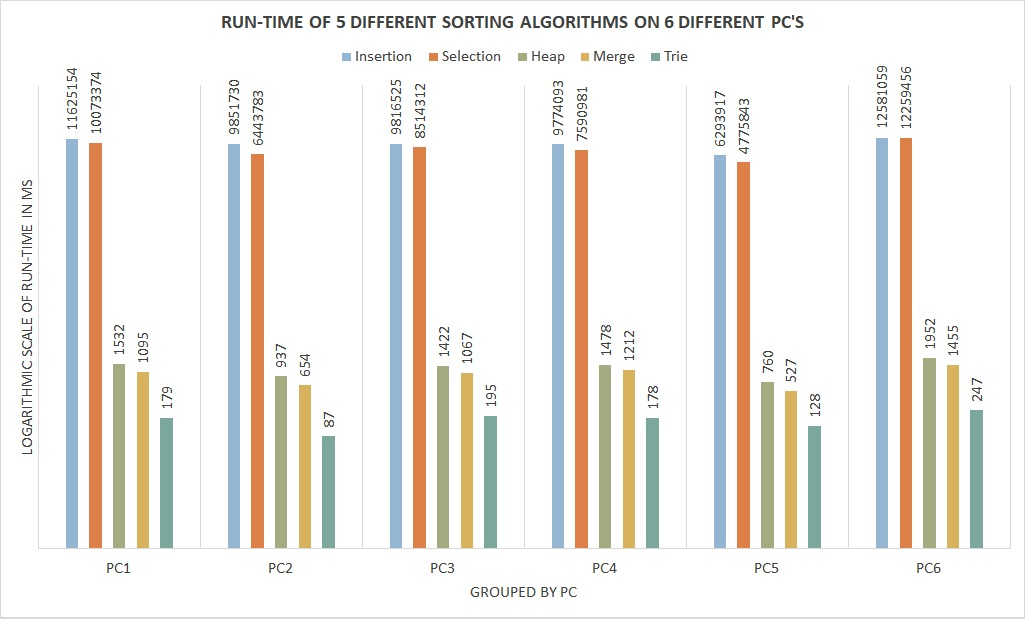
\includegraphics[width=1.2\textwidth]{figures/runtime1.jpg}}
  \caption{Logarithmic scale representation of the algorithms run-runtime on the six PCs.}
  \label{fig:pic1}
\end{figure}
In figure~\ref{fig:pic1} above, which is made from the data presented in table~\ref{tab:timings1} on page~\pageref{tab:timings1} it is clear to see both the run-time of each sorting algorithm and the apparent jumps between the time complexity for all the PCs. 

\vspace{0.5cm}
\subsection{Measurements on varying data amounts}
\label{sec:4.2}
As mentioned we decided to run all algorithms on the same PC with varying amounts of data to be able to make more direct comparisons between the five algorithms. The data used to create the following diagrams can be seen in table~\ref{tab:PC2timings} on page~\pageref{tab:PC2timings}. 
\begin{figure}[H]
  \makebox[\textwidth][c]{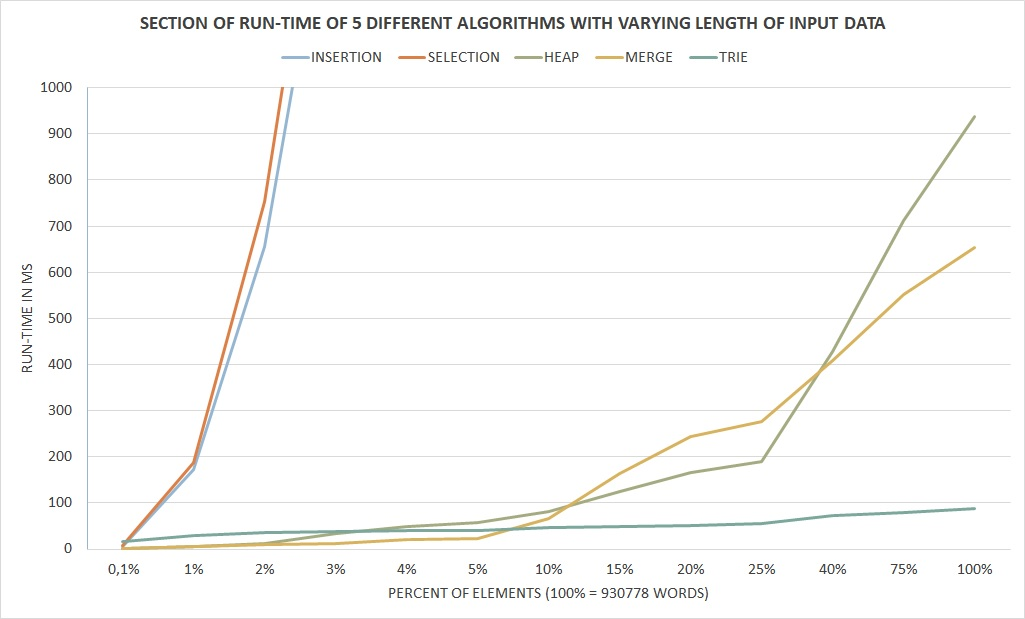
\includegraphics[width=1.1\textwidth]{figures/runtime2.jpg}}
  \caption{Timings ranging from 2ms to 1000ms. 100\% equals 930778 words}
  \label{fig:pic2}
\end{figure}

\begin{figure}[H]
  \makebox[\textwidth][c]{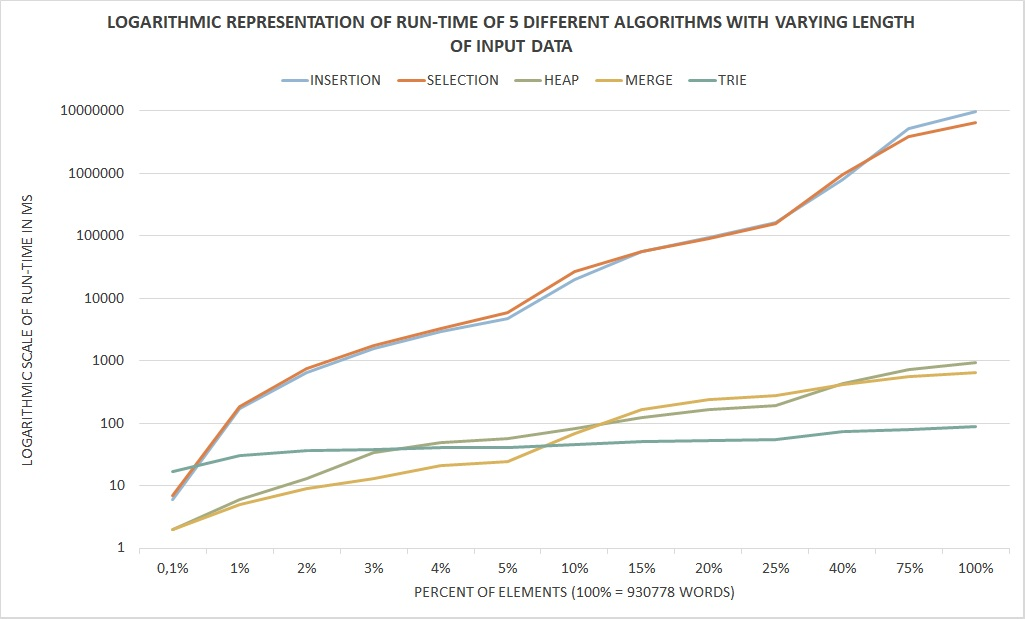
\includegraphics[width=1.1\textwidth]{figures/runtime3.jpg}}
  \caption{All timings represented on a logarithmic scale. 100\% equals 930778 words}
  \label{fig:pic3}
\end{figure}

Figure~\ref{fig:pic2} shows a smaller section of the timings in order to be able to see all the sorting algorithm graphs clearly, with the varying data amounts. This representation of the data is useful for an overall view of the differences, but in order to compare further we need to look at a logarithmic diagram. 
\\
Figure~\ref{fig:pic3} shows all of the timing data on a logarithmic scale with the varying data amounts. On a graph represented on a logarithmic scale, as in figure~\ref{fig:pic3}, the distinction between the efficiency for small amounts of data become more clear.







 

\vspace{0.5cm}
\section{Discussion} \label{discussion}

In this section we aim to compare the findings collected in our two tests with the known time complexity of the sorting algorithms. As well as talking about different use cases for the algorithms with the worst time complexity among the ones we have tested earlier.

\vspace{0.5cm}
\subsection{Discussion of results and scope}
\label{sec:5.1}


In figure~\ref{fig:pic1} on page~\pageref{fig:pic1} it is quite clear to see that for all the PCs, the relative jump between the time complexities is the same. The hardware does have a small impact on the run-time, but that difference is minuscule compared to the difference between the linear and linearithmic growth and between the linearithmic and quadratic growth. Even if we compare the fastest sorting algorithm on the slowest PC (Trie sort on PC6, run-time of \emph{247ms}), with the next-fastest algorithm on the fastest PC (Merge sort on PC5, run-time of \emph{527ms}), we still see more than a doubling of the run-time from the Trie sort to the Merge sort. The jump from any of the linearithmic algorithms to the quadratic algorithms would clearly never be solved by better hardware.
\\
\\
In figure~\ref{fig:pic2} on page~\pageref{fig:pic2} we can see an overall distinction between the three different time complexities and the graphs look similar to graphs shown for educational purposes. \cite{bigOgraph}. There is a clear difference in efficiency of the algorithms as the input data grows with the quickest and greatest efficiency loss for the to quadratic algorithms. The Trie sort algorithm with linear growth almost seems to loose very little efficiency as the data amount grows. 
\\
\\
In figure~\ref{fig:pic3} on page~\pageref{fig:pic3} we get a more clear view of the efficiency of the five sorting algorithms compared to each other. The 0.1\% of data amounts to 930 words and around this data size all other algorithms are more efficient than the linear time Trie sort. It is interesting that even the quadratic algorithms have a greater efficiency than the Trie when the data amount is this small. This is likely due to the amount of preprocessing in the Trie.
\\
\\
Based on the figures~\ref{fig:pic2} and \ref{fig:pic3} it is clear that Selection sort and Insertion sort will always have a greater efficiency loss than Merge and Heap sort - as well as Tries after the data set reaches a certain size. However both Selection and Insertion sort have some very useful properties, which can be used in a few different scenarios.
\\
Selection sort is a basic quadratic algorithm which is rarely used. Although it might never be used to sort a whole data set, it's possible to make use of one of its unique properties. If the algorithm is run only N times on an array of data, instead of sorting the whole array, then the first N elements will always be sorted and in their final position based on the final sorted array, while the remaining elements will remain unsorted \cite{sortingAlgo}. As an example suppose Selection sort is run 5 times on this array of integers:\\
\\
\([5, 2, 7, 12, 9, 11, 1, 1, 9, 34, 7, 0]\)\\
\\
The result would then be:\\
\\
\([\textbf{0, 1, 1, 2, 5}, 11, 12, 7, 9, 34, 7, 9]\)\\
\\
The first five entries are sorted and in their correct position, as if the whole array had been sorted.
This property can be useful in specific use cases. A use case could for example be a search engine like Google, where an arbitrary search such as "Sorting Algorithms" return 58 million results, but only the 10 most relevant will be shown on page one. 
In this scenario, running a Selection sort 10 times on the results, rather than sorting the whole result list with any of the other discussed algorithms, might result in a faster loading speed \cite{sortingAlgo}.
\\
\\
Insertion sort is another basic quadratic algorithm, however if it's used to sort an already sorted or nearly sorted array of data, then its time complexity becomes linear \cite{algo} \emph{page 250}. Because of this it might be possible to combine Insertion sort with a faster algorithm such as Merge or Heap sort. As an example Merge sort could be used to sort the data set to a nearly sorted state and then use insertion sort to finish the sorting, which in theory should speed up the sorting and save some memory use. In addition Insertion sort have a property similar to Selection sort. If it is run N times on an array of data then the first N elements will be sorted, but compared to Selection sort they will not be first N elements of the final sorted array. This can be useful if the use case is sorting of elements which is received from a data stream and they need to be kept sorted in real time \cite{sortingAlgo}.


\vspace{0.5cm}
\subsection{Reflection}
\label{sec:5.3}

The measurements of the different run-times in our two tests could have been optimized greatly. We have implemented a very basic stopwatch class in Java and we measured the timings from inside the IDE. Furthermore we could have run the sorting algorithms several hundred times instead of the few times they ran. 
\\
Practically this was not feasible, even though we would have gotten results that could be used to find standard deviation and mean which would have made outliers apparent, since all computers used for the measurements were our own personal PCs. For a more thorough examination we would follow the advice from Sesoft's paper on \emph{Microbenchmarks in Java and C\#}. \cite{sesoft}
\newline
Another interesting thing to measure, could be to implement the  algorithms in more programming languages beside Java and compare the run time of these implementations.  


\vspace{0.5cm}
\subsection{Conclusion}
\label{sec:5.4}
The time complexity have a direct impact on the run-time and efficiency of the different algorithms we examined. We saw the same pattern across all PCs in the hardware test. Even with a comparison of Merge sort on the fastest PC and with Trie sort on the slowest PC, showed that the difference in time complexity have a much greater impact on the run-time. 
\\
\\
We also noticed that the algorithms with a greater time complexity, such as the quadratic algorithms, are faster than the linear Trie sort if used on a small data set. The quadratic growth first starts to become a greater efficiency loss than the linear growth after a certain data amount. This can be utilized in a use case with a guaranteed small amount of data to achieve greater sorting efficiency.   


%%%%%%%%%%%%%%%%%%%%%%%%%%%%%%%%%%%%%%
% \newpage
% \section{NEW SECTION} \label{NAME}
% \input{sections/NAME.tex} 

%%%%%%%%%%%%%%%%%%%%%%%%%%%%%%%%%%%%%%
\label{EndOfText}

\newpage
\pagenumbering{roman} 
% \addcontentsline{toc}{section}{List of Figures}
\fancyfoot[C]{Page \thepage\ of \pageref{endOfDoc}}

% \listoffigures
% \thispagestyle{fancy}

% \newpage

% \addcontentsline{toc}{section}{List of Tables}
% \listoftables
% \thispagestyle{fancy}

\newpage
\addcontentsline{toc}{section}{References}
\bibliography{document.bib} 

\bibliographystyle{ieeetr}

\label{endOfDoc}
\end{document}